%% gtile_part.tex
\newpage
\subsection{Glass Tile}

\paragraph{Beschreibung des Filters aus Nutzersicht}

Dieses Filter lässt das Bild erscheinen, als würde es durch eine Wand aus Glasbausteinen betrachtet werden. Das Filter kann auf die aktive Ebene oder eine im Bild befindliche Auswahl angewendet werden.\footnote{\url{http://docs.gimp.org/de/plug-in-glasstile.html}} Die Kachelbreite und Kachelhöhe sind individuell einstellbar.

\paragraph{Algorithmus}

%Pseudocode, visuell
\begin{algorithm}[h]
\caption{Pseudo-Code des \glqq Glass Tile\grqq-Algorithmus}
\label{algo:gtile}
\begin{algorithmic}[1]
\State $xhalf \gets tileWidth  / 2$
\State $yhalf \gets tileHeight / 2$
\State $xplus \gets tileWidth  \mod 2$
\State $yplus \gets tileHeight \mod 2$
\State $ymiddle \gets 0$
\State $yoffs \gets 0$
\ForAll{$rows$ $r$ $\in input$}
	\State $ypixel2 \gets ymiddle + yoffs * 2$
	\State lese Zeile $ypixel2$ aus dem Eingabebild
	\State $yoffs$++
	\If{$yoffs = yhalf$}
		\State{$ymiddle \gets ymiddle + tileHeight$}
		\State{$yoffs \gets - (yhalf + yplus)$}
	\EndIf
	\State $xmiddle \gets 0$
	\State $xoffs \gets 0$
	\ForAll{$columns \in column$}
		\State $xpixel1 \gets (xmiddle + xoffs)$
		\State $xpixel2 \gets (xmiddle + xoffs * 2)$
		\State schreibe Pixel $xpixel2$ aus Eingabezeile nach $xpixel1$ in Ausgabezeile
		\State $xoffs$++
		\If{$xoffs = xhalf$}
			\State{$xmiddle \gets xmiddle + tileWidth$}
			\State{$xoffs \gets - (xhalf + xplus)$}
		\EndIf
	\EndFor
	\State speichere Ausgabezeile an Zeilenposition $r$ im Ausgabebild
\EndFor	
\end{algorithmic}
\end{algorithm}

%Beschreibung Algorithmus allgemeinsprachlich
\begin{figure}[h]
\begin{center}
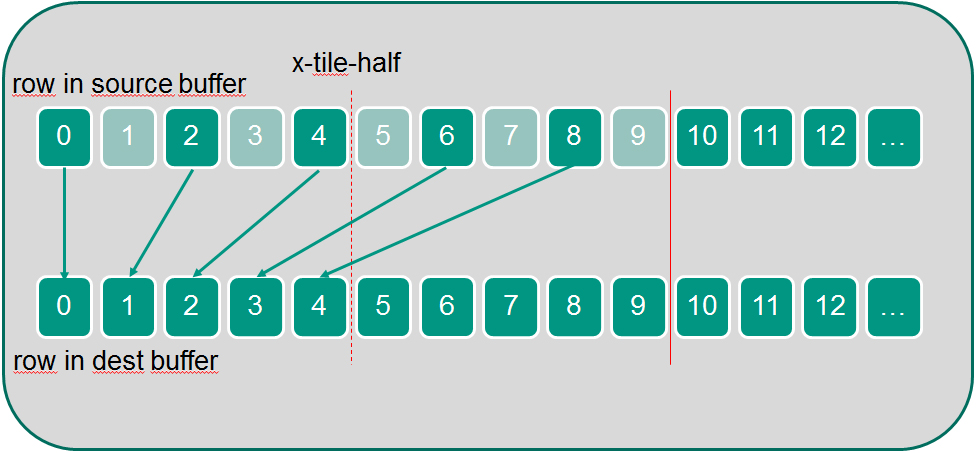
\includegraphics[width=0.95\textwidth]{gtile1.png}
\end{center}
\caption{Verrückung der Spalten innerhalb einer Zeile}\label{fig:gtile1}
\end{figure}
Der Algorithmus erzeugt sowohl zeilenweise als auch spaltenweise eine Verrückung und Wiederholung innerhalb der Kacheln. Dabei wird jede zweite Zeile in einer Kachel hintereinander in die erste Hälfte der Kachel verschoben wie in Abbildung~\ref{fig:gtile1} zu sehen.\newline
\begin{figure}[h]
\begin{center}
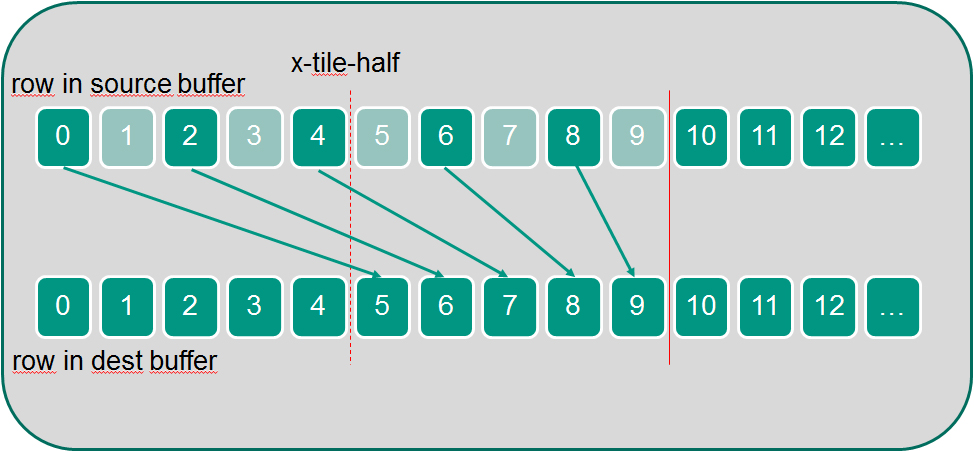
\includegraphics[width=0.95\textwidth]{gtile2.png}
\end{center}
\caption{Wiederholung der verrückten Spalten innerhalb einer Kachelzeile}\label{fig:gtile2}
\end{figure}
Diese gelesenen und verschobenen Zeilen werden anschließend in der zweiten Hälfte nochmals wiederholt, was in Abbildung~\ref{fig:gtile2} dargestellt ist.\newline
Die Verrückung und Wiederholung der Spalten erfolgt analog. Auf diese Weise wird Kachel für Kachel bearbeitet. Der sequentielle original Algorithmus liest dabei komplette Zeilen ein und führt darauf die notwendigen Spaltenverschiebungen durch.

\paragraph{Portierung}
Die Portierung basiert auf einem Area Filter. Wegen des speziellen Gegl-Frameworks, das Kacheln arbitrarer Größe zur Bearbeitung liefert, war es notwendig die Initialisierung der für den Algorithmen relevanten Variablen anzupassen, insbesondere \emph{ymiddle}, \emph{yoffs}, \emph{xmiddle} und \emph{xoffs}, da es möglich ist, dass die linke obere Ecke des zu bearbeitenden Gegl-Tiles nicht kongruent mit dem fortlaufenden Glass-Tile ist, und die Operation irgendwo zufällig in der Mitte einer Glass-Tile beginnen kann.

\paragraph{Parallelisierung}
Da alle Pixel theoretisch unabhängig voneinander und in beliebiger Reihenfolge betrachtet und bearbeitet werden können, von der Indizierung für die korrekte Verschiebung abgesehen, wäre eine logische Schlussfolgerung, dass der Algorithmus trivial parallelisierbar ist. Jedoch hat sich erst nach einer Testimplementierung gezeigt, dass die einzelnen Kopiervorgänge zwar unabhängig voneinander sind, jedoch Memory-Effekte wie z.B. Cache-Ausnutzung jeglichen Speedup wieder zunichte machen. Dies lässt sich darauf begründen, dass der Berechnungsaufwand pro Pixel gesehen werden kann und vernachlässigbar ist, da weder Bedingungen geprüft werden, noch kostenintensive Rechenoperationen durchgeführt werden, und somit lediglich ein Kopiervorgang stattfindet. Somit lohnt sich eine generisch implementierte Parallelisierung nicht, und es bleibt Gegenstand zur Untersuchung, ob durch eine hardwarespezifische Implementierung ein Speedup erreicht werden kann.\newline
Dennoch wurde eine Parallelisierung mittels OpenMP realisiert, bei der die zu bearbeitenden Zeilen gleichmäßig auf die vorhandenen Threads aufgeteilt werden.